\PassOptionsToPackage{usenames}{xcolor}
\PassOptionsToPackage{dvipsnames}{xcolor}
\documentclass[11pt,a4paper,twoside,final,titlepage,openright,fleqn]{book}%
\usepackage{beamerarticle}

\usepackage[utf8]{inputenc}
\usepackage[T1]{fontenc}
\usepackage[spanish]{babel}

\usepackage{listings}
\usepackage{palatino}
\usepackage{lmodern}

%\renewcommand*\rmdefault{lmr}
%\renewcommand*\ttdefault{ppl}

\usepackage{url}
\usepackage{multicol}

\usepackage{tabularx}

\usepackage{tikz}
\usetikzlibrary{positioning}
\usetikzlibrary{arrows}
\usetikzlibrary{mindmap}

\usepackage{pgfplots}
\pgfplotsset{compat=1.5}

\usepackage{ccicons}

\tikzset{
  invisible/.style={opacity=0},
  visible on/.style={alt=#1{}{invisible}},
  alt/.code args={<#1>#2#3}{%
    \alt<#1>{\pgfkeysalso{#2}}{\pgfkeysalso{#3}} % \pgfkeysalso doesn't change the path
  },
  bloque/.style={rectangle,draw=black, top color=white, bottom color=blue!50,
                 very thick, inner sep=0.5em, minimum size=0.6cm, text centered, font=\tiny},
  bloquelibre/.style={rectangle,draw=black, top color=white, bottom color=blue!10,
                 very thick, inner sep=0.5em, minimum size=0.6cm, text centered, font=\tiny},
  flecha/.style={->, >=latex', shorten >=1pt, thick},
  etiqueta/.style={text centered, font=\tiny} 
}



\usepackage[a4paper,left=2cm,right=2cm,top=2.5cm,bottom=4cm]{geometry}
\usepackage[colorlinks=true,linkcolor=blue,citecolor=blue,urlcolor=blue,plainpages=false,bookmarksnumbered=true,pdfpagemode=UseOutlines]{hyperref}


\usepackage[nottoc]{tocbibind}

%\usepackage[fixlanguage]{babelbib}


\usepackage{graphicx}
\usepackage{xcolor}
\usepackage{tikz}
\usetikzlibrary{arrows,positioning} 

\newcommand{\textgood}[1]{%
{\color{blue!60!black}\textbf{#1}}%
}

\newcommand{\textbad}[1]{%
{\color{red!80!black}\textbf{#1}}%
}

\newcommand{\textmark}[1]{%
{\color{orange!70!black}\textbf{#1}}%
}

\newcommand{\textenum}[1]{%
{\color{blue!60!black}\textbf{#1}}%
}

\newcommand{\textemph}[1]{%
{\color{green!40!black}\textbf{#1}}%
}

\newcommand{\versionid}{2021.1}
\newcommand{\versiondate}{Noviembre de 2021}

\newcommand{\coursetitle}{Programación en concurrente en C++ moderno}
\newcommand{\moduleintro}{Introducción a la concurrencia}
\newcommand{\modulehilos}{Hilos}

\newcommand{\pppbook}{\emph{Programming: Principles and Practice using C++, 2$^a$ edición~\cite{stroustrup:2014}}}
\newcommand{\cppbook}{\emph{The C++ Programming Language, 4$^a$ edición~\cite{stroustrup:2013}}}
\newcommand{\tourbook}{\emph{A tour of C++, 2$^a$ edición~\cite{stroustrup:2018}}}


\newtheorem{ejer}{Ejercicio}

\usepackage{url}

\usepackage{pdfpages}

\usepackage{todonotes}

%Package fancyhdr
\usepackage{fancyhdr}
\setlength{\headheight}{1.7cm}%{13.6pt}
\pagestyle{fancyplain}
\fancyhf{}
\lhead{
\includegraphics[height=1.25cm]{logos/uc3m.png}}
\chead{}
\rhead{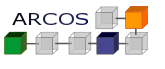
\includegraphics[height=1.25cm]{logos/arcos.png}}
\rfoot{\begin{tabular}{r}\coursetitle\\Versión \versionid\end{tabular}}
\cfoot{\begin{tabular}{c}{\thepage}\\{}\end{tabular}}
\lfoot{
\begin{tabular}{l}
\textbf{\ccbysa} -- CC BY-SA 4.0\\J. Daniel Garcia -- ARCOS@UC3M
\end{tabular}
}
\renewcommand{\headrulewidth}{0.5pt} % remove lines as well
\renewcommand{\footrulewidth}{0.5pt}
\renewcommand{\plainheadrulewidth}{0.5pt}
\renewcommand{\plainfootrulewidth}{0.5pt}

\renewcommand{\topfraction}{0.9}
\renewcommand{\textfraction}{0.1}
\renewcommand{\floatpagefraction}{0.9}

\usepackage{palatino}
\usepackage{lmodern}

\renewcommand*\rmdefault{lmr}
\renewcommand*\ttdefault{ppl}

\makeindex

\begin{document}

\mode<article>{
\lstset{
  language=C++,
  belowcaptionskip=1\baselineskip,
  breaklines=true,
  xleftmargin=\parindent,
  showstringspaces=false,
  basicstyle=\small,
  keywordstyle=\bfseries\color{green!40!black},
  commentstyle=\itshape\color{purple!40!black},
  identifierstyle=\color{blue},
  stringstyle=\color{brown},
  columns=fullflexible,
  inputencoding=utf8,
  extendedchars=true,
  upquote=true,
  morekeywords=[1]{_Pragma,constexpr,nullptr,alignof,alignas,decltype,override,final,noexcept,deprecated,thread_local,co_await,co_return,co_yield,fallthrough},
  literate=%
    {¿}{{?`}}{1}
    {¡}{{!`}}{1}
    {á}{{\'a}}{1}
    {é}{{\'e}}{1}
    {í}{{\'i}}{1}
    {ó}{{\'o}}{1}
    {ú}{{\'u}}{1}
    {ñ}{{\~n}}{1}
}
}

\mode<presentation>{
\lstset{
  language=C++,
  belowcaptionskip=1\baselineskip,
  breaklines=true,
  xleftmargin=\parindent,
  showstringspaces=false,
  basicstyle=\scriptsize,
  keywordstyle=\bfseries\color{green!40!black},
  commentstyle=\itshape\color{purple!40!black},
  identifierstyle=\color{blue},
  stringstyle=\color{orange},
  directivestyle=\bfseries\color{green!40!black},
  columns=fullflexible,
  inputencoding=utf8,
  extendedchars=true,
  upquote=true,
  morekeywords=[1]{_Pragma,constexpr,nullptr,alignof,alignas,decltype,override,final,noexcept,deprecated,thread_local,co_await,co_return,co_yield,fallthrough},
  literate=%
    {¿}{{?`}}{1}
    {¡}{{!`}}{1}
    {á}{{\'a}}{1}
    {é}{{\'e}}{1}
    {í}{{\'i}}{1}
    {ó}{{\'o}}{1}
    {ú}{{\'u}}{1}
    {ñ}{{\~n}}{1}
}
}

\newcommand{\cppkey}[1]{%
{\color{green!40!black}\textbf{#1}}%
}

\newcommand{\cppid}[1]{%
{\color{blue}\textbf{#1}}%
}

\newcommand{\cppstr}[1]{%
{\color{orange}\textbf{#1}}%
}


\lstdefinestyle{terminal}{
  language=bash,
  basicstyle=\scriptsize\ttfamily,
  numbersep=3pt,
  frame=tb,
  columns=fullflexible,
  backgroundcolor=\color{yellow!20},
}



\frontmatter

\pagestyle{empty}
\begin{titlepage}
\tikz[remember picture,overlay] \draw [fill,Blue] (current page.north west) rectangle +(0.2\paperwidth,-\paperheight);
\begin{flushright}

\includegraphics[width=5cm]{logos/uc3m.png}
\\
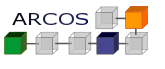
\includegraphics[width=5cm]{logos/arcos.png}
\end{flushright}

\vfill

\begin{tabular}{p{3cm}l}
&
\LARGE{Material de curso}
\\

&\\

&
\LARGE{\coursetitle}
\\

&\\

&
Version: \versionid
\\

&
\versiondate
\\

\end{tabular}
\vfill
\begin{tabular}{p{3cm}l}
&José Daniel García Sánchez\\
&Departamento de Informática\\
&Grupo ARCOS\\
&Universidad Carlos III de Madrid\\
&Av. Universidad, 30\\
&28911 Leganés, Madrid\\
&\url{josedaniel.garcia@uc3m.es}\\
\end{tabular}
\vspace{1cm}
\\
\begin{tabular}{p{3cm}l}
&
%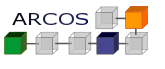
\includegraphics[width=5cm]{logos/arcos.png}
%\includegraphics[width=8cm]{logos/logo-uc3m.jpg}
\\
\end{tabular}
\end{titlepage}

\pagestyle{fancyplain}
\chapter*{Atribución-CompartirIgual 4.0 Internacional (CC BY-SA 4.0)}

Este es un resumen legible por humanos (y no un sustituto) de la
(código legal disponible en
\url{https://creativecommons.org/licenses/by-sa/4.0/legalcode}
).

\section*{Usted es libre de:}

\begin{itemize}

\item \textbf{Compartir} --
copiar y redistribuir el material en cualquier medio o formato.

\item \textbf{Adaptar} -- 
remezclar, transformar y construir a partir del material
para cualquier propósito, incluso comercialmente.

\end{itemize}

La licenciante no puede revocar estas libertades en tanto usted siga los
términos de la licencia.

\section*{Bajo los siguientes términos:}

\begin{itemize}

\item \ccAttribution \quad \textbf{Atribución} --
Usted debe dar crédito de manera adecuada, brindar un enlace a la licencia, e
indicar si se han realizado cambios. Puede hacerlo en cualquier forma
razonable, pero no de forma tal que sugiera que usted o su uso tienen el apoyo
de la licenciante. 

\item \ccShareAlike \quad \textbf{CompartirIgual} --
Si remezcla, transforma o crea a partir del material, debe distribuir su
contribución bajo la lamisma licencia del original. 

\item \textbf{No hay restricciones adicionales} -- 
No puede aplicar términos legales ni medidas tecnológicas que restrinjan
legalmente a otras a hacer cualquier uso permitido por la licencia. 

\end{itemize}

\section*{Avisos:}

No tiene que cumplir con la licencia para elementos del materiale en el dominio
público o cuando su uso esté permitido por una excepción o limitación
aplicable.

No se dan garantías. La licencia podría no darle todos los permisos que
necesita para el uso que tenga previsto. Por ejemplo, otros derechos como
publicidad, privacidad, o derechos morales pueden limitar la forma en que
utilice el material.


\cleardoublepage
\chapter*{Presentación}

Bienvenidos al curso de programación concurrente en C++ moderno.


\section*{Structure}

Los contenidos de este curso se estructuran de la siguiente forma:

\begin{enumerate}

\item \ldots

\end{enumerate}

\cleardoublepage
\chapter*{Agradecimientos}

En primer lugar, me gustaría dar las gracias a Bjarne Stroustrup
por darnos el lenguaje de programación C++.

También me gustaría expresar mi gratitud a todos los miembreos del
grupo de trabajo ISO/IEC JTC1/SC22/WG21, que han trabajado durante
décadas para mejorar y actualizar el lenguaje.
La discusión con muchos de ellos sobre diversos aspectos específicos
del lenguaje y de la biblioteca estándar han sido para mi de gran utilidad.

Así mismo, me gustaría agradecer de forma especial a todos aquellos
que han proporcionado realimentación sobre versiones previas de este 
material.


\cleardoublepage
\tableofcontents
\todototoc
\listoftodos

\mainmatter

\pagestyle{fancyplain}
\mode<article>{\chapter{\moduleintro}}

\mode<presentation>{\begin{frame}[shrink=20]{Licencia Creative Commons}

\begin{tabularx}{.98\textwidth}{lX}
\ccLogo & Este trabajo se distribuye bajo licencia
Atribución-NoComercial-SinDerivadas 4.0 Internacional (CC BY-NC-ND 4.0).\\

&\\

& \multicolumn{1}{c}{\textbf{Usted es libre de}:}\\

&\\

&
\textbf{Compartir} --
copiar y redistribuir el material en cualquier medio o formato.
\\

&\\

& \multicolumn{1}{c}{\textbf{Bajo los siguientes términos}:}\\

&\\

\ccAttribution &
Atribución -- Usted debe dar crédito de manera adecuada, brindar un enlace a la licencia, e indicar si se han realizado cambios. Puede hacerlo en cualquier forma razonable, pero no de forma tal que sugiera que usted o su uso tienen el apoyo de la licenciante.
\\

\ccNonCommercialEU &
NoComercial -- Usted no puede hacer uso del material con propósitos comerciales. 
\\

\ccNoDerivatives &
SinDerivadas -- Si remezcla, transforma o crea a partir del material, no podrá distribuir el material modificado. 
\\

\end{tabularx}

\end{frame}
}
\section{Concurrencia en C++}

\begin{frame}[t]{Motivación}
\begin{itemize}
  \item C++ ofrece un modelo de concurrencia propio.

  \mode<presentation>{\vfill\pause}
  \item Cualquier implementación que cumple el estándar debe proporcionarlo.
    \begin{itemize}
      \item \textmark{Portabilidad} de código concurrente: Windows, POSIX, ...
      \item Resuelve \textmark{problemas} inherentes a PThreads.
    \end{itemize}

  \mode<presentation>{\vfill\pause}
  \item Implicaciones:
    \begin{itemize}
      \item Reglas en el \textemph{lenguaje}.
      \item Funcionalidades en la \textemph{biblioteca estándar}.
    \end{itemize}

  \mode<presentation>{\vfill\pause}
  \item Influencia sobre C11 (ISO/IEC 9899:2011).

  \mode<presentation>{\vfill\pause}
  \item \textbad{Importante}: Concurrencia y paralelismo son conceptos relacionados pero distintos.
\end{itemize}
\end{frame}

\begin{frame}[t]{Estructura}
\begin{itemize}
  \item El \textemph{lenguaje} ofrece:
    \begin{itemize}
      \item Un nuevo modelo de memoria.
      \item Almacenamiento local al hilo (\cppkey{thread\_local}).
    \end{itemize}

  \mode<presentation>{\vfill\pause}
  \item La \textemph{biblioteca} ofrece:
    \begin{itemize}
      \item Tipos \textmark{atómicos}.
        \begin{itemize}
          \item Útiles para programación libre de cerrojos de forma portable.
        \end{itemize}
      \item \textmark{Abstracciones} portables para la concurrencia.
        \begin{itemize}
          \item \textmark{Hilos}: \cppid{thread} \cppid{jthread}.
          \item \textmark{Exclusión mutua}: \cppid{mutex}, \cppid{mutex\_*}.
          \item \textmark{Gestión de bloqueos}: \cppid{unique\_lock}, \cppid{lock\_guard}, 
                                                \cppid{scoped\_lock}, \ldots
          \item \textmark{Notificación}: \cppid{condition\_variable}, \ldots
          \item \textmark{Semáforos}: \cppid{counting\_semaphore}, \cppid{binary\_semaphore}.
          \item \textmark{Barreras}: \cppid{latch}, \cppid{barrier}.
          \item \textmark{Resultados de hilos}: \cppid{packaged\_task}, \cppid{future},
                                                \cppid{promise}, \ldots
        \end{itemize}
    \end{itemize}
\end{itemize}
\end{frame}


\section{Hilos}

\begin{frame}[t,fragile]{Lanzamiento de hilos}
\begin{itemize}
  \item Un hilo representado por la clase \cppid{std::thread}.
    \begin{itemize}
      \item Normalmente representa un hilo del SO.
    \end{itemize}
\begin{lstlisting}
void f1();
void f2();

void g() {
  std::thread t1{f1}; // Lanza un hilo que ejecuta f1()
  std::thread t2{f2}; // Lanza un hilo que ejecuta f2()

  t1.join(); // Espera a que t1 termine.
  t2.join(); // Espera a que t2 termine.
}
\end{lstlisting}
\end{itemize}
\end{frame}

\begin{frame}[t,fragile]{Objetos función}
\begin{itemize}
  \item Un \textgood{objeto función} es un tipo de datos que puede compartarse
        como una función.
\begin{lstlisting}[escapechar=@]
struct mi_funcion {
  mi_funcion(int x) : valor{x} {}
  void operator()() { procesa(valor_); }
  int valor_;
};

void test() {
  mi_funcion f{42};
  f(); // Ejecuta f.operator()()
  //...@\pause@
  std::thread t1(f); // Ejecuta f.operator()() en t1
  std::thread t2(mi_funcion{42}); // Sobre un temporal
  //...
  t1.join();
  t2.join();
}
\end{lstlisting}

\end{itemize}
\end{frame}

\begin{frame}[t,fragile]{Objetos compartidos}
\begin{itemize}
  \item Dos hilos pueden acceder a un objeto compartido.
  \item Posibilidad de carreras de datos.
\end{itemize}
\begin{lstlisting}
int x = 42;

void f() { ++x; }
void g() { x=0; }
void h() { cout << "Hola" << endl; }
void i() { cout << "Adios" << endl; }

void carrera() {
  std::thread t1{f}; std::thread t2{g};

  t1.join(); t2.join();

  std::thread t3{h}; std::thread t4{i};

  t3.join(); t4.join();
}
\end{lstlisting}
\end{frame}

\begin{frame}[t,fragile]{Paso de argumentos}
\begin{itemize}
  \item Paso de parámetros simplificado sin necesidad de \emph{casts}.
  \item Varias alternativas.
\end{itemize}

\begin{columns}[T]

\column{.3\textwidth}

\begin{lstlisting}
void f1(int x);

struct f2 {
  void operator()();
  f2(int px) : x{px} {}
  int x;
}

void f3(double x);
\end{lstlisting}

\column{.7\textwidth}
\begin{lstlisting}
void g() {
  std::thread t1{f1, 10}; // Ejecuta f1(10)
  std::thread t2{f2{20}}; // Ejecuta f2{20}.operator()()
  std::thread t3{[] { f3(1.5); } }; // Ejecuta una lambda

  t1.join();
  t2.join();
  t3.join();
}
\end{lstlisting}

\end{columns}

\end{frame}

\begin{frame}[t,fragile]{Comprobación de argumentos}
\begin{itemize}
  \item Se comprueba número y tipo de los argumentos.
\end{itemize}

\mode<presentation>{\vfill}
\begin{block}{Paso de argumentos}
\begin{lstlisting}
void f1(int x);
void f2(double x, double y);

void g() {
  std::thread t1{f1, 10}; // Ejecuta f1(10)
  std::thread t2{f1}; // Error
  std::thread t3{f2, 1.0} // Error
  std::thread t4{f2, 1.0, 1.0}; // Ejecuta f2(1.0,1.0)
  //...
  // Joins de hilos
\end{lstlisting}
\end{block}
\end{frame}

\section{Acceso a datos compartidos}

\begin{frame}[fragile]{Exclusión mutua}
\begin{itemize}
  \item Un \cppid{std::mutex} permite controlar el acceso con exclusión mutua a un recurso.

    \begin{itemize}
      \item \cppid{lock()}: Adquiere el cerrojo asociado.
      \item \cppid{unlock()}: Libera el cerrojo asociado.
    \end{itemize}
\end{itemize}

\mode<presentation>{\vfill}
\begin{columns}[T]
\begin{column}{.5\textwidth}
\begin{block}{Uso de mutex}
\begin{lstlisting}
std::mutex m;
int x = 0;

void f() {
  m.lock();
  ++x;
  m.unlock();
}
\end{lstlisting}
\end{block}
\end{column}

\begin{column}{.5\textwidth}
\begin{block}{Lanzamiento de hilos}
\begin{lstlisting}
void g() {
  std::thread t1(f); 
  std::thread t2(f);
  t1.join(); 
  t2.join();
  cout << x << "\n";
}
\end{lstlisting}
\end{block}
\end{column}
\end{columns}

\end{frame}

\begin{frame}[t,fragile]{Problemas con \texttt{lock()}/\texttt{unlock()}}
\begin{itemize}
  \item \textenum{Posibles problemas}:
    \begin{itemize}
      \item Olvido de \textbad{liberar cerrojo}.
      \item \textbad{Excepciones}.
    \end{itemize}
\end{itemize}

\mode<presentation>{\vfill}
\begin{columns}[T]
\begin{column}{.5\textwidth}
\begin{block}{Olvidos}
\begin{lstlisting}
std::mutex m;
int x = 0;

void f() {
  m.lock();
  ++x;
  // Ouch! olvido liberar cerrojo
}
\end{lstlisting}
\end{block}
\end{column}

\mode<presentation>{\pause}

\begin{column}{.5\textwidth}
\begin{block}{Excepciones}
\begin{lstlisting}
std::mutex m;
int x = 0;

void f() {
  m.lock();
  g(x); // Excepciones?
  m.unlock();
}
\end{lstlisting}
\end{block}
\end{column}
\end{columns}
\end{frame}

\begin{frame}[t,fragile]{Evitando problemas con \texttt{unique\_lock}}
\begin{itemize}
  \item Solución: \cppid{unique\_lock}.
    \begin{itemize}
      \item \textgood{Patrón}: \textmark{RAII} (Resource Acquisition Is Initialization).
    \end{itemize}
\end{itemize}

\mode<presentation>{\vfill}
\begin{columns}[T]
\begin{column}{.5\textwidth}
\begin{block}{Cerrojo automático}
\begin{lstlisting}
std::mutex m;
int x = 0;

void f() {
  // Adquiere el cerrojo
  std::unique_lock l{m}; 
  g(x);
} // Libera el cerrojo
\end{lstlisting}
\end{block}
\end{column}

\begin{column}{.5\textwidth}
\begin{block}{Lanzamiento de hilos}
\begin{lstlisting}
void g() {
  std::thread t1(f); 
  std::thread t2(f);
  t1.join(); 
  t2.join();

  std::cout << x << "\n";
}
\end{lstlisting}
\end{block}
\end{column}
\end{columns}
\end{frame}


\begin{frame}[fragile]{Adquisición de múltiples \texttt{mutex}}
\begin{itemize}
  \item Un \cppid{scoped\_lock} permite adquirir varios \cppid{mutex} a la vez.
    \begin{itemize}
      \item Adquiere todos o ninguno.
      \item Si alguno está bloqueado espera dejando libres todos.
    \end{itemize}
\begin{lstlisting}
mutex m1, m2, m3;
void f() {
  // Otras operaciones

  {
    std::scoped_lock l{m1,m2,m3};
    // Acceso a datos compartidos
  }

  // Otra operaciones

} // Se liberan m1, m2, m3
\end{lstlisting}
\end{itemize}
\end{frame}

\section{Esperas}

\begin{frame}[t,fragile]{Esperas de tiempo}
\begin{itemize}
  \item Acceso al reloj.
\begin{lstlisting}
using namespace std::chrono;
auto t1 = high_resolution_clock::now();
\end{lstlisting}
  \item Diferencia de tiempos.
\begin{lstlisting}
auto dif = duration_cast<nanoseconds>(t2-t1);
cout << dif.count() << endl;
\end{lstlisting}
  \item Especificación de una espera.
\begin{lstlisting}
using namespace std::literals;
std::this_thread::sleep_for(500ms);
\end{lstlisting}
\end{itemize}
\end{frame}

\begin{frame}[t,fragile]{Variables condición}
\begin{itemize}
  \item Mecanismo para sincronizar hilos en acceso a recursos compartidos.
    \begin{itemize}
      \item \cppid{wait()}: Espera en un \cppid{mutex}.
      \item \cppid{notify\_one()}: Despierta a un hilo en espera.
      \item \cppid{notify\_all()}: Despierta a todos los hilos en espera.
    \end{itemize}
\begin{block}{Productor/Consumidor}
\begin{lstlisting}
class peticion;

std::queue<peticion> cola; // Cola de peticiones
std::condition_variable cv; // Variable condición
std::mutex m;

void productor();
void consumidor();
\end{lstlisting}
\end{block}
\end{itemize}
\end{frame}

\begin{frame}[t,fragile]
\begin{columns}

\begin{column}{.5\textwidth}
\begin{block}{Consumidor}
\begin{lstlisting}
void consumidor() {
  for (;;) {
    std::unique_lock l{m};

    while (cola.empty()) {
      cv.wait(l);
    }

    auto p = cola.front();
    cola.pop();
    l.unlock();
   
    procesa(p);
  };
}
\end{lstlisting}
\end{block}
\end{column}

\begin{column}{.5\textwidth}
\begin{itemize}
  \item Efecto de \cppid{wait}:
    \begin{enumerate}
      \item Libera el cerrojo y espera una notificación.
      \item Adquiere el cerrojo al despertarse.
    \end{enumerate}
\end{itemize}
\end{column}

\end{columns}
\end{frame}

\begin{frame}[t,fragile]
\begin{columns}
\begin{column}{.5\textwidth}
\begin{block}{Productor}
\begin{lstlisting}
void productor() {
  for (;;) {
    peticion p = genera();

    unique_lock<mutex> l{m};
    cola.push(p);

    cv.notify_one();
  }
}
\end{lstlisting}
\end{block}
\end{column}

\begin{column}{.5\textwidth}
\begin{itemize}
\item Efecto de \cppid{notify\_one()}:
  \begin{enumerate}
    \item Despierta a uno de los hilos esperando en la condición.
  \end{enumerate}
\end{itemize}
\end{column}

\end{columns}
\end{frame}


\section{Tareas asíncronas}

\begin{frame}[t]{Tareas asíncronas y futuros}
\begin{itemize}
  \item Una tarea asíncrona permite el lanzamiento simple de la ejecución de una tarea:
    \begin{itemize}
      \item En otro hilo de ejecución.
      \item Como una tarea diferida.
    \end{itemize}

  \mode<presentation>{\vfill\pause}
  \item El lanzamiento de una tarea asíncrona devuelve un \cppid{std::future}.

  \mode<presentation>{\vfill\pause}
  \item Un futuro \cppid{f} tiene una operación \cppid{f.get()}
    \begin{itemize}
      \item Si un hilo devuelve un valor, la operación \cppid{get()} devuelve ese valor.
      \item Si un hilo lanza una excepción, la operación \cppid{get()} lanza esa excepción.
    \end{itemize}
\end{itemize}
\end{frame}

\begin{frame}[t,fragile]{Invocación de tareas asíncronas}
\begin{lstlisting}
#include <future>
#include <iostream>

double tarea(int i, int j);

int main() {
  std::future<double> r = std::async(tarea, 1, 10);
  std::future<double> s = std::async(tarea, 50, 100);
  otra_tarea();
  auto x = r.get();
  auto y = r.get();
  std::cout << "x = " << x << "\n";
  std::cout << "y = " << y << "\n";
  return 0;
}
\end{lstlisting}
\end{frame}

\mode<article>{
  \section{Lecturas recomendadas}

\begin{enumerate}

\item .

\end{enumerate}

  \section{Ejercicios}

\begin{enumerate}

\item .

\end{enumerate}

}



\nocite{*}
\bibliographystyle{abbrv}
\bibliography{bib/cppref}

\end{document}
